\documentclass[conference]{IEEEtran}
\IEEEoverridecommandlockouts
% The preceding line is only needed to identify funding in the first footnote. If that is unneeded, please comment it out.
\usepackage{cite}
\usepackage{amsmath,amssymb,amsfonts}
\usepackage{algorithmic}
\usepackage{graphicx}
\graphicspath{ {img/} }
\usepackage{hyperref}
\hypersetup{
    hidelinks
}
\usepackage{textcomp}
\usepackage{xcolor}
\usepackage{wrapfig}
\def\BibTeX{{\rm B\kern-.05em{\sc i\kern-.025em b}\kern-.08em
    T\kern-.1667em\lower.7ex\hbox{E}\kern-.125emX}}
\begin{document}

\title{Computer Technology Project I\\
{\large TurtleBot3 - Robot Design}
\thanks{Identify applicable funding agency here. If none, delete this.}
}

\author{\IEEEauthorblockN{Daniel Pihl}
\IEEEauthorblockA{\textit{Århus University} \\
AU712814}
\and
\IEEEauthorblockN{Steffen Petersen}
\IEEEauthorblockA{\textit{Århus University} \\
AU722120}
}

\maketitle

\begin{abstract}
Define what have we done and talked about in the report.\\
Set up the general "question" for the report to answer.\\
\end{abstract}

\begin{IEEEkeywords}
component, formatting, style, styling, insert
\end{IEEEkeywords}

\section{Introduction}
In this project, our main goal was to implement a Turtlebot3 robot for a simulated version of search and rescue purposes.\\
This would involve creating a program to allow the robot to move autonomously and avoid obstacles, utilizing the 
Robot Operating System (ROS), all while searching for targets on the floor.\\
We also aim to optimize this robot for the highest possible speed, through an efficient navigation logic, 
following the "see - think - act" concept.\\


\section{Specifications}
\subsection{TurtleBot3 Burger}
In this project we are using the TurtleBot3 Burger robot, to practice our ROS based robot programming.\\
The TurtleBot3 Burger is equipped with a Raspberry Pi 3 Model B \cite{b1} in combination with an OpenCR 1.0 board, to 
provide us with options for programming and controlling it. \\

\subsection{LDS-01 LIDAR}
Additionally the Burger has an LDS-01\cite{b2} Lidar scanner mounted on top, which we use for the navigation of the Burger.\\


\subsection{Raspberry Pi 3 Model B}
The Raspberry Pi is a small-scale computer ideal for hobbyist purposes, with GPIO pins, that we could use to add extra sensors to
our robot \cite{b3}.\\


\subsection{RGB Sensor}
Using the extra IO support of the Raspberry PI, we could add the ISL-29125 RGB sensor \cite{b4}, that allows us to simulate scanning for
victims.\\


\section{Process}
In this section we will elaborate on the process of developing our own understanding of the problem, and the solutions we have 
come up with along the way.\\
\subsection{Design and Implementation}
In this section we are going to talk about our own thoughts on design and implementation but in an abstract way.\\
Concrete implementation and thoughts will come in the later sections. \\
\vspace*{2pt}\\
In the early stages of our process, we started out with the RGB sensor as it was a component that just had to be mounted 
on the robot and connected to the Pi. If we could make that work, it was a simple matter of just implementing it later.\\
Our intention was to make the sensor read some coloured tags from the floor, which would simulate victims that our robot 
had to recognize as it moves around.\\
Firstly we installed the necessary libraries on the Pi, \textit{smbus} to communicate with the sensor, and \textit{time} for 
the initialization. \\
To start working on the implementation, we were given a template, that already had the code for communicating through 
\textit{smbus} with the sensor, to configure the registers of the sensor. We then had to add to that, a way to extract the red, 
green and blue values from the registers within the sensor, so that we could use these in our to-be robot code, and detect 
victims.\\
After we got the RGB sensor working we moved on to theorize what implementation we wanted to use for navigation with the robot.\\
Our Turtlebot3 was equipped with a LIDAR sensor which is capable of scanning 360° with a laser, that could measure distance. 
It would return data in the form of an array like so:
\[dist = \left[d_0, d_1, ..., d_{359}\right]\]
Where $d_i$ is the distance to nearest object at $i$ degrees from the front of the sensor, going counterclockwise. 
In the first implementation we would simply look at a span of $120^{\circ}$ that we would divide into three subcategories:
\[left = \left[d_{60}, d_{59}, ..., d_{15}\right], N = 45\]
\[front = \left[d_{14}, d_{13}, ..., d_0, d_{359}, d_{358}, ..., d_{345}\right], N = 30\]
\[right = \left[d_{344}, d_{343}, ..., d_{300}\right], N = 45\]

The reason we chose to only look forwards, was due to us thinking it would be smarter for the robot
to simply turn instead of having to go backwards, since this would allow the robot to achieve an overall 
higher average linear speed. \\
Using these cones, we would have to specify what the robot would do in different cases, 
which we implemented with if/else statements. Each of the abstract cases can be seen in the illustrations below. 
Note that in Case 1, we would ideally make a sharp swing turn, instead of reversing out of the corner.
\begin{figure}[h] %this figure will be at the left
    \centering
    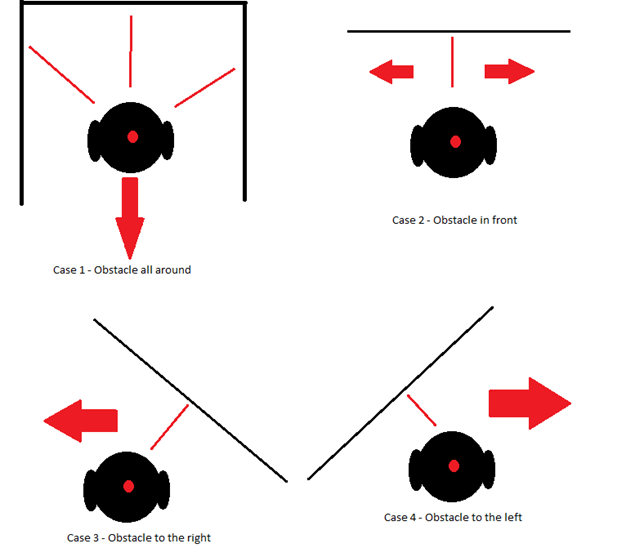
\includegraphics[width=0.5\textwidth]{cases.png}
    \caption{Theoretical cases for navigation}
\end{figure} 

Moving on, we could now get to work practically with the real robot, and at first we would need to set up ROS and 
get familiar with it, before running our own code on it. Up until now it had all been mostly theoretical, 
which would only get us so far.\\
ROS is a necessary tool to help us control the robot. In short it is a collection 
of tools, libraries and conventions that allows us to simplify the creation of complex and robust robot behavior.\\
Having ROS installed, we needed to get to know it, and to that end we followed a tutorial. We downloaded the 
Turtlebot3 packages to set up a virtual environment using ROS features, where we would be able to drive a simulation 
of a turtle around a little screen with our keyboard. \\

From here on and till the end of our timeframe, we continuously worked on the Robots navigation and optimization.
We were presented with a sort of starter build of the code \cite{b5} for our robot's obstacle avoidance.\\
The task at hand first was to update the given code and make the robot read from a different 
span of angles using the LIDAR. \\
\vspace*{2pt}\\
At first we wanted to implement a way to read from angles -45° to 45° to 
represent left and right. The current aim was to design according to the following picture\cite{b6}
\begin{figure}[h] %this figure will be at the left
    \centering
    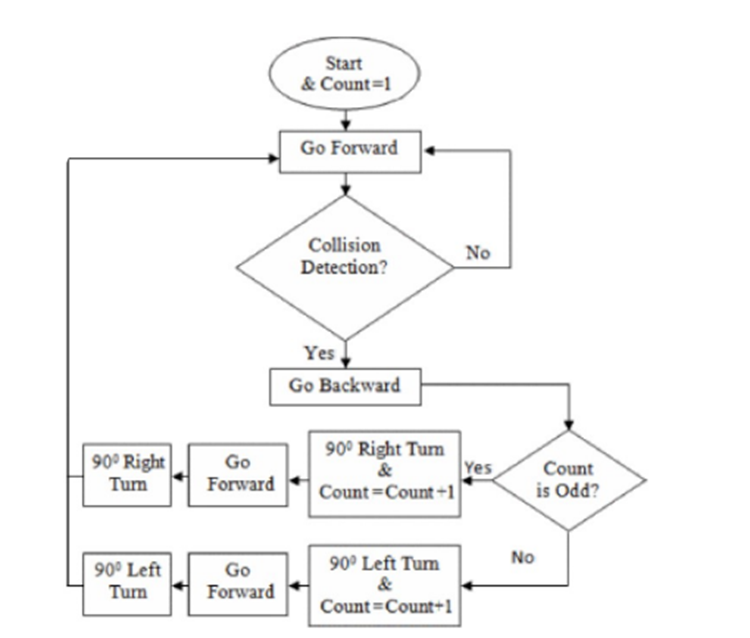
\includegraphics[width=0.5\textwidth]{initialNav.png}
    \caption{Simple navigation logic}
\end{figure} 
We got the simple navigation to work and wanted to implement a reading from both Lidar and the RGB sensor 
in a frequency that made sense. After we got the basics down, had a robot that could do simple maneuvering 
and send relevant data from both Lidar and RGB sensor, it was time to optimize the navigation further.\\
We would start by optimizing how the robot navigates and move on to optimizing the linear speed, where we had 
to consider the linear speed vs the angular speed. In short, if we were to move faster forwards, we wouldn't be 
able to make a sharp turn due to the higher speed. Likewise, if we must make a sharp turn, we won't be able to have 
very high speed.\\
To achieve a higher linear speed whilst turning would want to break the turn into smaller steps. 
If our robot would be facing an obstacle, we want to calculate how much it should turn. Instead of making 
the entire turn in one go, we wanted to apply half of the angle and store how much angle there is left 
to apply it at the next publishing to complete the entire turn. See the following two pictures. \cite{b7}\\
\begin{figure}[h] %this figure will be at the left
    \centering
    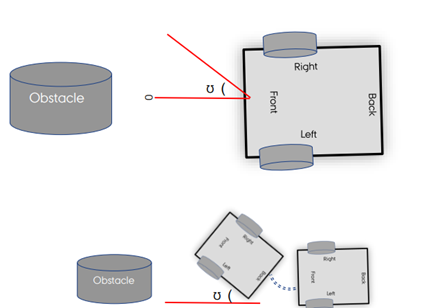
\includegraphics[width=0.4\textwidth]{betterNav1.png}
\end{figure}\\
\begin{figure}[h] %this figure will be at the left
    \centering
    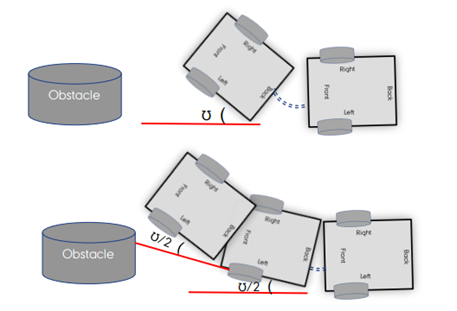
\includegraphics[width=0.4\textwidth]{betterNav2.png}
    \caption{Speed Optimization for turns}
\end{figure} \\
By doing this, we would in theory be able to always achieve a higher linear velocity whilst still avoiding 
obstacles in our way.\\
The final two things we wanted to implement was a way to calculate the average linear speed and to optimize 
that so we would have the highest possible linear speed over the course of the time our robot was driving, 
and a collision counter, which would increment if the distance to an obstacle was lower or equal to 4cm for 
the front of the robot or 5cm for other angles.\\
Our goal was to keep the linear speed as high as possible and the collision counter as low as possible.


\subsection{Experiment setup and Results}
\subsubsection{Method}
During our process of making the program for the robot, we have been using a reiterated model called the waterfall model.
This model is perfect for the structure of our project. Firstly, we would analyze the requirements. \\
Then we make decisions based on how we think the robot should operate in different situations (System Design).\\
Then we would make an implementation of our code (Implementation), and lastly, test the implementation by 
letting the robot run, and observing it (Testing). Whatever failures we might find with the program, 
we could then reiterate the process by either going back to system design, if our design choices were wrong, 
or go to change the implementation if it simply behaved unexpectedly. See the following illustration.\\
\vspace{4cm}\\
\begin{figure}[h] %this figure will be at the left
    \centering
    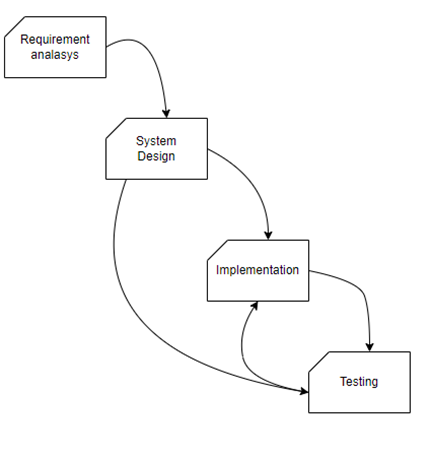
\includegraphics[width=0.4\textwidth]{waterfallmodel.png}
    \caption{Waterfall Model (selfmade illu.)}
\end{figure} 
\\
\subsubsection{ROS Setup}
As previously mentioned, before we could begin truly working with the actual robot, we needed some abstraction in place, 
in this case ROS.\\
ROS allows us to use packages that have previously been used for working with this robot platform, 
and then quite simply customize our own node that can run our implementations of code. \\
To familiarize ourselves with the workings of ROS, we did start by running through the tutorial of 
virtually running a simulation using the different features of ROS. Learning the uses for ROS topics, packages, 
nodes and messages.\\
\vspace*{2pt}\\
In practice, we used the turtlebot3\_example and \\turtlebot3\_bringup packages from the turtlebot3 repository \cite{b8}. \\
The bringup package contained a launch file that ensured the necessities for the turtlebot3 would be running, 
starting the LIDAR and ROScore. On top of this, we could use the turtlebot3\_example's turtlebot3\_obstacle node 
to serve as a base for our own implementation of obstacle avoidance and navigation.\\
\vspace*{2pt}\\
This was handy as it already had the code for setting up the Twist message from geometry\_msgs and a topic to allow 
us to control the motors on the robot simply using this premade message.\\
Additionally it had an example of how to read the data from our LIDAR, also setting up a listener for the scan message, 
from the LaserScan package.\\
That was about the end of what we kept from the example however, as the actual implementation of the \textit{obstacle()} function 
is completely changed, both in terms of principle and code. Additionally we did modify the \textit{get\_scan()} function, 
though it's principally similar. The main difference, is that we changed how the filter worked, as invalid readings 
in our implementation should not be set to 0.
\\
\vspace*{2pt}\\
\subsubsection{Test setup}
Following the waterfall model, we would need to test each implementation of code, to determine what changes should be made.\\
We set up a little obstacle course made from cardboard boxes to function as walls, and some red paper dots on the ground 
to simulate victims to be found. Our idea was the robot should navigate collision free whilst moving around without either 
getting stuck in a loop where it would go in circles, or just getting stuck overall. \\
The robot initially had a few problems with the course. The first struggle was it would register itself too close to an 
obstacle and immediately try to turn, but as it turned a new obstacle would be spotted and it would only move a little 
bit before turning again, creating a zig-zag effect. \\Another problem arose when we tried fixing the first problem, that 
it would simply get too close to an obstacle and then get stuck on a wall because we turned too late. \\
Our optimization and final solutions follow in the next section.
\\
\vspace*{2pt}\\
\subsubsection{Optimization}
In our first system design, the idea was that we wanted to maintain the linear speed constant throughout, and simply 
decide to turn more or less depending on how close we were to an obstacle. \\
We attempted this by partitioning the LIDARs view, as we have illustrated below, into a front cone and 2 cones on both 
the left and right side of the bot. \\
\begin{figure}[h] %this figure will be at the left
    \centering
    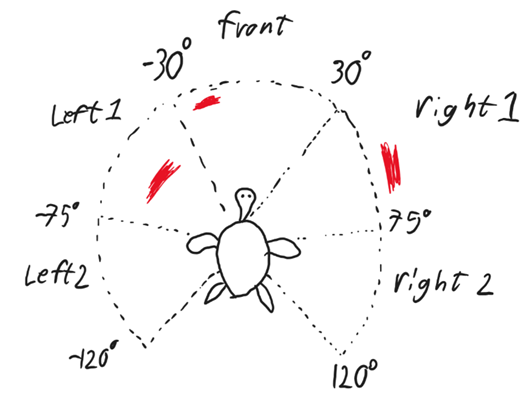
\includegraphics[width=0.5\textwidth]{turtleExample.png}
    \caption{Design showcase and Example}
\end{figure} \\
In the illustration we have also included some red blobs to explain a scenario where these are obstacles. \\
We would only decide to turn if something was in the front cone, as we would otherwise be able to continue. 
When an obstacle was found in front, we would evaluate if there was more room on the left or right side of the bot, 
to decide which way we should turn. In this case we would turn right, as the left has the closer obstacle. 
To determine how much we would turn, we then had different cases, where we first determine if “Left 1” has an 
object within a certain distance, and if it didn't we would check “Left 2”. The amount to turn was then determined 
by a constant (different from “Left 1” to “Left 2”) plus a variable fraction, based on the distance to the obstacle. 
This allowed the amount we turned to be relative to how close an obstacle was, which should in theory give us smoother turns.
\\\\
This implementation however, took many iterations and wasn't quite working, we found the bot would be too stubborn with 
going forward, and unable to avoid obstacles if it ever got into a corner that was too tight. 
This would likely be because the decision for turning would be too narrowly minded, as we don't have a 
full mapping of the terrain, just deciding based on which side had the closer wall. 
This would eventually get it to turn into corners, but turn too little to avoid a wall on the right, 
when the left wall was just a little closer. We needed a new edge case to deal with being cornered.
\\\\
During the later iterations, we noticed some strange decisions from the bot, and decided to add some debugging print
statements, to allow us to see which cones saw what. At this moment we realized we had in fact messed up the cones 
relative to the LIDAR, as we had reversed it entirely, assuming that the array of data from the LIDAR would be ordered 
chronologically with the direction it spins. \\
However this turned out to not be the case, and it was in fact reversed. 
Still we decided to rework the principles on which it should turn slightly. \\
Moving to the next iteration, we would instead only evaluate ±90° from the front, 
still keeping the front cone, but only using one left and right cone, 
and still maintaining the fraction based turn decisions. \\
Of course here we would also add solutions to combat getting stuck in a corner, even if this meant slowing down or backing up slightly. 
This was done by adding a new check, to determine if there was an obstacle very close to an even narrower front cone, at just ±15°, 
this would usually only be triggered if a previous turn had put our nose close to another wall. 
In this case we would stop moving forward, and simply continue turning until our entire front-cone 
was cleared of any immediate obstacles. This of course sacrifices a good bit 
of the average linear speed, however it felt like it was the better option compared to getting stuck. 
Additionally we did add another measure if we ended up being truly stuck, by counting the number of repeated turn decisions, 
if we repeated the same loop too often, we decided it likely meant we were stuck on a corner, as had been observed during testing, 
and then we could reverse out of this situation, to make a new decision instead.
\\\\
\subsubsection{Program design}
Our program has its roots in the Turtlebot3\_example package \cite{b5}, using a similar structure for the \textit{Obstacle} class,
additionally we added the simple RGB Sensor class from our previous work, to initialize the sensor for use in the main loop.
\\\\
Below we will describe the details of our obstacle avoidance loop, and what each iteration goes through.
\begin{itemize}
\item \textbf{Get LIDAR data}\\
Starting off each loop, we must get a new reading from the LIDAR to be able to navigate with current positional data.\\
For this we have the \textit{get\_scan()} function, which is quite similar in structure to the one from the template.
\begin{figure}[h] %this figure will be at the left
    \centering
    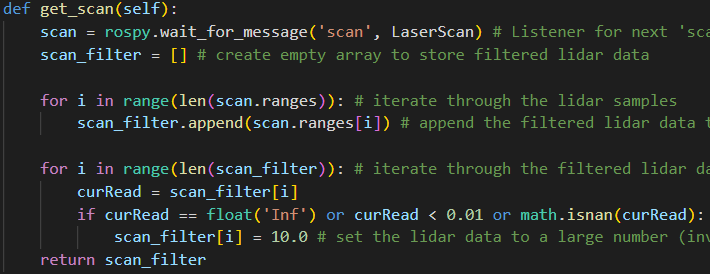
\includegraphics[width=0.5\textwidth]{get_scan.png}
    \caption{\textit{get\_scan()} function}
\end{figure} \\
We listen for a new message from the LIDAR and then proceed to filter this data sorting out 
values like infinity, 0 and NaN, setting these entries to 10 instead, which we know is not going to affect our navigation.\\
\item \textbf{Sort and Evaluate Data}\\
Having received the filtered data from the \textit{get\_scan()} function, we need to organize it and evaluate it,
to be able to use it for navigation.
\begin{figure}[h] %this figure will be at the left
    \centering
    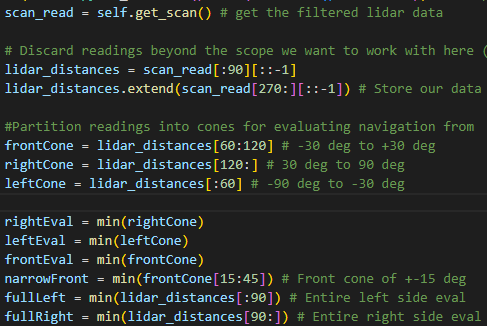
\includegraphics[width=0.5\textwidth]{evaluateAndSort.png}
    \caption{Organize data}
\end{figure} \\
We do this by creating a new array, intended to store our readings in order from left to right, starting at -90 degrees up 
to 90 degrees. Since our LIDAR returns an array of 360 readings, one from each degree of angle, we take the first 90 
readings which are on the left side of the bot, and reverse this, because it by default is stored right to left.
And we then add to that, the final 270th reading up to the 360th reading, which would be on the right side of the bot, also 
reversing this.\\
After this we simply use the new array, to create cones for viewing zones of the bot, and then proceeed to store the readings of
shortest distance in each of these relevant areas, to use for evaluation in our navigation.\\
\item \textbf{Check for Victims}\\
In order to check for victims, we read the current red and blue values from the RGB sensor, as the tags we are looking for a red,
we know to look for a higher value of red and lower value of blue. These new values are compared to an older baseline value, 
to avoid reading double. The first baseline is made in initialization of the obstacle avoidance loop.
\begin{figure}[h] 
    \centering
    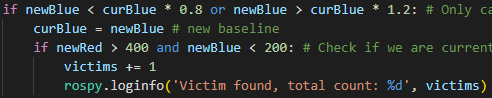
\includegraphics[width=0.5\textwidth]{victimCheck.png}
    \caption{Victim searching code}
\end{figure} \\
We've decided that 20\% was a good amount to allow the readings to fluctuate, and whenever it has changed more than this,
it's because we've either travelled over a tag we need to read, or we've just come off a tag we've already read. This means
we can create a new baseline here, to compare future readings with. When this happens, we need to also check if we did come across
a new tag, or if we went off of one, so this is where we use the new readings from the sensor, to determine if we are over a red 
tag, and if so increment our counter.\\
\item \textbf{Check for collision}\\
Checking for collisions we need to evaluate on the LIDAR readings, we've decided to simplify the check quite a lot, and
so we simply check if the robot is within 5cm + the LIDAR error. 
\begin{figure}[h] 
    \centering
    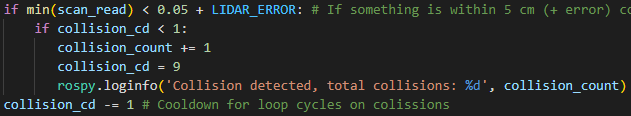
\includegraphics[width=0.5\textwidth]{collisionCheck.png}
    \caption{Collision counter code}
\end{figure} \\
To avoid any double counting, we have implemented a cooldown 
counter, that decreases with every loop-cycle, so we shouldn't read multiple collisions in the same corner, 
as we would be gone by then. \\
\item \textbf{Navigation control}\\
The navigation controls consists of a few steps, firstly we need to check for a flag to see if we have been marked as 
cornered from a previous loop, and if so, we must continue to turn until our front-cone is clear of immediate obstacles.
\begin{figure}[h] 
    \centering
    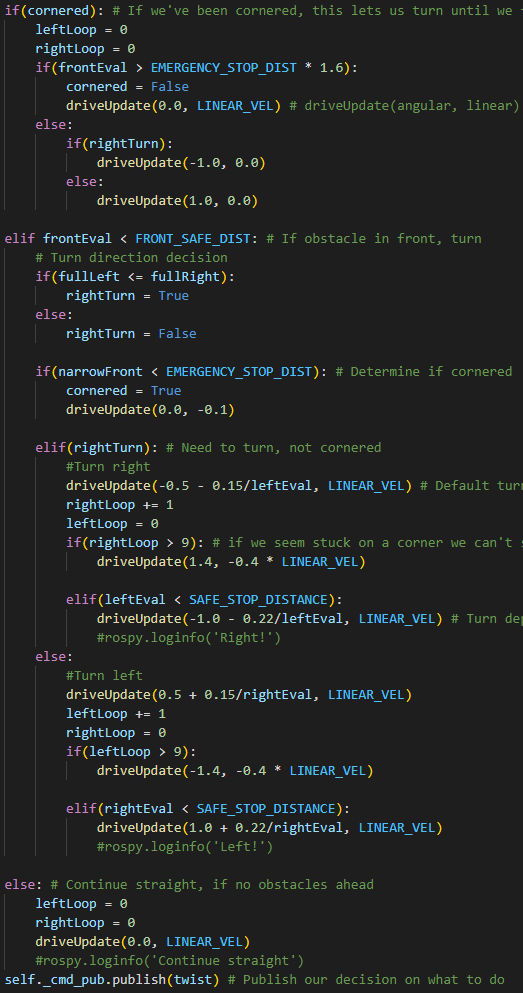
\includegraphics[width=0.5\textwidth]{Navigation.png}
    \caption{Navigation code}
\end{figure} \\
If we haven't been marked as stuck, we can move on to see, if there are obstacles in front of us, within our set FRONT\_SAFE\_DIST,
and if we are clear, we jump to the else case, which simply lets us continue forward at full speed. \\
Should we instead have obstacles, we need to turn to avoid them, so we immediately decide which way we need to turn, comparing
the evaluation variable for the left side, to the right side, and storing the decision in another flag called rightTurn.\\
Moving on, we check our narrow front cone, for any very close obstacles, this is to make sure we have room to turn at all, and if
we don't, we set the cornered flag and proceed to back up slightly, and the next n-loops would then keep us turning until we are
clear to move forward. \\
If all instead goes well, and our narrow front is clear, we either go to the left or right turn case depending on the flag, 
and here we firstly have a default case that updates the Twist message variables through \\\textit{driveUpdate(angular, linear)},
to a small turn. \\
We then move on to check if the obstacle is within our set SAFE\_STOP\_DISTANCE, to determine if we should turn more than the
default. If we should, we set a new driveUpdate, with a variable amount of turning, depending on the distance to the nearest obstacle.\\
The final detail of the control loop, is that we have added counters to check for repeated entries into the turning loops. This is
to combat getting stuck on corners, so if we enter the same loop to many times in a row, we are most likely stuck, and so we 
reverse instead of continuing to turn into the wall.\\
Once all of the above has been executed, we have the correct Twist message values as is updated by the \textit{driveUpdate(a, l)}
function, and so we can publish these to ROS and thus make the robot drive according to our control logic.\\
\item \textbf{Update variables}\\
To finalize the loop, we just need to keep track of the average speed of the robot, this is done using the linear speed we've
saved to the twist.message and a simply counter for how many loops we've been through.
\begin{figure}[h] 
    \centering
    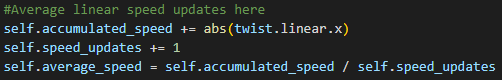
\includegraphics[width=0.5\textwidth]{averageSpeed.png}
    \caption{Continous update of average speed}
\end{figure} 


\end{itemize}


\subsection{Abbreviations and Acronyms}\label{AA}
Define abbreviations and acronyms the first time they are used in the text, 
even after they have been defined in the abstract. Abbreviations such as 
IEEE, SI, MKS, CGS, ac, dc, and rms do not have to be defined. Do not use 
abbreviations in the title or heads unless they are unavoidable.

\subsection{Units}
\begin{itemize}
\item Use either SI (MKS) or CGS as primary units. (SI units are encouraged.) English units may be used as secondary units (in parentheses). An exception would be the use of English units as identifiers in trade, such as ``3.5-inch disk drive''.
\item Avoid combining SI and CGS units, such as current in amperes and magnetic field in oersteds. This often leads to confusion because equations do not balance dimensionally. If you must use mixed units, clearly state the units for each quantity that you use in an equation.
\item Do not mix complete spellings and abbreviations of units: ``Wb/m\textsuperscript{2}'' or ``webers per square meter'', not ``webers/m\textsuperscript{2}''. Spell out units when they appear in text: ``. . . a few henries'', not ``. . . a few H''.
\item Use a zero before decimal points: ``0.25'', not ``.25''. Use ``cm\textsuperscript{3}'', not ``cc''.)
\end{itemize}

\subsection{Equations}
Number equations consecutively. To make your 
equations more compact, you may use the solidus (~/~), the exp function, or 
appropriate exponents. Italicize Roman symbols for quantities and variables, 
but not Greek symbols. Use a long dash rather than a hyphen for a minus 
sign. Punctuate equations with commas or periods when they are part of a 
sentence, as in:
\begin{equation}
a+b=\gamma\label{eq}
\end{equation}

Be sure that the 
symbols in your equation have been defined before or immediately following 
the equation. Use ``\eqref{eq}'', not ``Eq.~\eqref{eq}'' or ``equation \eqref{eq}'', except at 
the beginning of a sentence: ``Equation \eqref{eq} is . . .''

\subsection{\LaTeX-Specific Advice}

Please use ``soft'' (e.g., \verb|\eqref{Eq}|) cross references instead
of ``hard'' references (e.g., \verb|(1)|). That will make it possible
to combine sections, add equations, or change the order of figures or
citations without having to go through the file line by line.

Please don't use the \verb|{eqnarray}| equation environment. Use
\verb|{align}| or \verb|{IEEEeqnarray}| instead. The \verb|{eqnarray}|
environment leaves unsightly spaces around relation symbols.

Please note that the \verb|{subequations}| environment in {\LaTeX}
will increment the main equation counter even when there are no
equation numbers displayed. If you forget that, you might write an
article in which the equation numbers skip from (17) to (20), causing
the copy editors to wonder if you've discovered a new method of
counting.

{\BibTeX} does not work by magic. It doesn't get the bibliographic
data from thin air but from .bib files. If you use {\BibTeX} to produce a
bibliography you must send the .bib files. 

{\LaTeX} can't read your mind. If you assign the same label to a
subsubsection and a table, you might find that Table I has been cross
referenced as Table IV-B3. 

{\LaTeX} does not have precognitive abilities. If you put a
\verb|\label| command before the command that updates the counter it's
supposed to be using, the label will pick up the last counter to be
cross referenced instead. In particular, a \verb|\label| command
should not go before the caption of a figure or a table.

Do not use \verb|\nonumber| inside the \verb|{array}| environment. It
will not stop equation numbers inside \verb|{array}| (there won't be
any anyway) and it might stop a wanted equation number in the
surrounding equation.

\subsection{Some Common Mistakes}\label{SCM}
\begin{itemize}
\item The word ``data'' is plural, not singular.
\item The subscript for the permeability of vacuum $\mu_{0}$, and other common scientific constants, is zero with subscript formatting, not a lowercase letter ``o''.
\item In American English, commas, semicolons, periods, question and exclamation marks are located within quotation marks only when a complete thought or name is cited, such as a title or full quotation. When quotation marks are used, instead of a bold or italic typeface, to highlight a word or phrase, punctuation should appear outside of the quotation marks. A parenthetical phrase or statement at the end of a sentence is punctuated outside of the closing parenthesis (like this). (A parenthetical sentence is punctuated within the parentheses.)
\item A graph within a graph is an ``inset'', not an ``insert''. The word alternatively is preferred to the word ``alternately'' (unless you really mean something that alternates).
\item Do not use the word ``essentially'' to mean ``approximately'' or ``effectively''.
\item In your paper title, if the words ``that uses'' can accurately replace the word ``using'', capitalize the ``u''; if not, keep using lower-cased.
\item Be aware of the different meanings of the homophones ``affect'' and ``effect'', ``complement'' and ``compliment'', ``discreet'' and ``discrete'', ``principal'' and ``principle''.
\item Do not confuse ``imply'' and ``infer''.
\item The prefix ``non'' is not a word; it should be joined to the word it modifies, usually without a hyphen.
\item There is no period after the ``et'' in the Latin abbreviation ``et al.''.
\item The abbreviation ``i.e.'' means ``that is'', and the abbreviation ``e.g.'' means ``for example''.
\end{itemize}
An excellent style manual for science writers is \cite{b7}.

\subsection{Authors and Affiliations}
\textbf{The class file is designed for, but not limited to, six authors.} A 
minimum of one author is required for all conference articles. Author names 
should be listed starting from left to right and then moving down to the 
next line. This is the author sequence that will be used in future citations 
and by indexing services. Names should not be listed in columns nor group by 
affiliation. Please keep your affiliations as succinct as possible (for 
example, do not differentiate among departments of the same organization).

\subsection{Identify the Headings}
Headings, or heads, are organizational devices that guide the reader through 
your paper. There are two types: component heads and text heads.

Component heads identify the different components of your paper and are not 
topically subordinate to each other. Examples include Acknowledgments and 
References and, for these, the correct style to use is ``Heading 5''. Use 
``figure caption'' for your Figure captions, and ``table head'' for your 
table title. Run-in heads, such as ``Abstract'', will require you to apply a 
style (in this case, italic) in addition to the style provided by the drop 
down menu to differentiate the head from the text.

Text heads organize the topics on a relational, hierarchical basis. For 
example, the paper title is the primary text head because all subsequent 
material relates and elaborates on this one topic. If there are two or more 
sub-topics, the next level head (uppercase Roman numerals) should be used 
and, conversely, if there are not at least two sub-topics, then no subheads 
should be introduced.

\subsection{Figures and Tables}
\paragraph{Positioning Figures and Tables} Place figures and tables at the top and 
bottom of columns. Avoid placing them in the middle of columns. Large 
figures and tables may span across both columns. Figure captions should be 
below the figures; table heads should appear above the tables. Insert 
figures and tables after they are cited in the text. Use the abbreviation 
``Fig.~\ref{fig}'', even at the beginning of a sentence.

\begin{table}[htbp]
\caption{Table Type Styles}
\begin{center}
\begin{tabular}{|c|c|c|c|}
\hline
\textbf{Table}&\multicolumn{3}{|c|}{\textbf{Table Column Head}} \\
\cline{2-4} 
\textbf{Head} & \textbf{\textit{Table column subhead}}& \textbf{\textit{Subhead}}& \textbf{\textit{Subhead}} \\
\hline
copy& More table copy$^{\mathrm{a}}$& &  \\
\hline
\multicolumn{4}{l}{$^{\mathrm{a}}$Sample of a Table footnote.}
\end{tabular}
\label{tab1}
\end{center}
\end{table}

\begin{figure}[htbp]
\centerline{
\includegraphics{fig1.png}}
\caption{Example of a figure caption.}
\label{fig}
\end{figure}

Figure Labels: Use 8 point Times New Roman for Figure labels. Use words 
rather than symbols or abbreviations when writing Figure axis labels to 
avoid confusing the reader. As an example, write the quantity 
``Magnetization'', or ``Magnetization, M'', not just ``M''. If including 
units in the label, present them within parentheses. Do not label axes only 
with units. In the example, write ``Magnetization (A/m)'' or ``Magnetization 
\{A[m(1)]\}'', not just ``A/m''. Do not label axes with a ratio of 
quantities and units. For example, write ``Temperature (K)'', not 
``Temperature/K''.

\section*{Acknowledgment}

The preferred spelling of the word ``acknowledgment'' in America is without 
an ``e'' after the ``g''. Avoid the stilted expression ``one of us (R. B. 
G.) thanks $\ldots$''. Instead, try ``R. B. G. thanks$\ldots$''. Put sponsor 
acknowledgments in the unnumbered footnote on the first page.

\section*{References}

Please number citations consecutively within brackets \cite{b1}. The 
sentence punctuation follows the bracket \cite{b2}. Refer simply to the reference 
number, as in \cite{b3}---do not use ``Ref. \cite{b3}'' or ``reference \cite{b3}'' except at 
the beginning of a sentence: ``Reference \cite{b3} was the first $\ldots$''

Number footnotes separately in superscripts. Place the actual footnote at 
the bottom of the column in which it was cited. Do not put footnotes in the 
abstract or reference list. Use letters for table footnotes.

Unless there are six authors or more give all authors' names; do not use 
``et al.''. Papers that have not been published, even if they have been 
submitted for publication, should be cited as ``unpublished'' \cite{b4}. Papers 
that have been accepted for publication should be cited as ``in press'' \cite{b5}. 
Capitalize only the first word in a paper title, except for proper nouns and 
element symbols.

For papers published in translation journals, please give the English 
citation first, followed by the original foreign-language citation \cite{b6}.

\begin{thebibliography}{00}
\bibitem{b1} \raggedright Robotis e-Manual - TurtleBot3 Specifications, visited 03-05-2023, \url{https://emanual.robotis.com/docs/en/platform/turtlebot3/features/#specifications}.
\bibitem{b2} \raggedright Robotis e-Manual - LDS-01 Specifications, visisted 03-05-2023, \url{https://emanual.robotis.com/docs/en/platform/turtlebot3/appendix_lds_01/}
\bibitem{b3} \raggedright Raspberry Pi 3 Model B Documentation, visisted 03-05-2023, \url{https://www.raspberrypi.com/products/raspberry-pi-3-model-b/}
\bibitem{b4} \raggedright ISL-29125 RGB Sensor Datasheet, visisted 28-05-2023, \url{https://cdn.sparkfun.com/datasheets/Sensors/LightImaging/isl29125.pdf}
\bibitem{b5} \raggedright Turtlebot3 Package, template code, visisted 28-05-2023, \url{https://github.com/ROBOTIS-GIT/turtlebot3/blob/master/turtlebot3_example/nodes/turtlebot3_obstacle}
\bibitem{b6} \raggedright BrightSpace Week 7, Navigation Slides
\bibitem{b7} \raggedright Brightspace week 9, Speed Optimization Slides
\bibitem{b8} \raggedright Turtlebot3 master repository, visisted 28-05-2023, \url{https://github.com/ROBOTIS-GIT/turtlebot3/tree/master}

\end{thebibliography}
\vspace{12pt}
\color{red}
IEEE conference templates contain guidance text for composing and formatting conference papers. Please ensure that all template text is removed from your conference paper prior to submission to the conference. Failure to remove the template text from your paper may result in your paper not being published.

\end{document}
